\documentclass{article}
\usepackage{ae,aecompl}
\usepackage{todonotes}
\usepackage{chngcntr}
\usepackage{tikz-cd}
\usepackage{graphicx}
\graphicspath{ {./images/}}
\usepackage[all,cmtip]{xy}
\usepackage{amsmath, amscd}
\usepackage{amsthm}
\usepackage{amssymb}
\usepackage{amsfonts}
\usepackage{bm}
\usepackage{qsymbols}
\usepackage{latexsym}
\usepackage{mathrsfs}
\usepackage{mathtools}
\usepackage{cite}
\usepackage{color}
\usepackage{url}
\usepackage{enumerate}
\usepackage{verbatim}
\usepackage[draft=false, colorlinks=true]{hyperref}
\usepackage{pdfpages}
\usepackage[margin=1.2in]{geometry}
\usepackage{IEEEtrantools}

\usepackage{fancyhdr}


\usepackage[nameinlink]{cleveref}


\DeclareMathOperator*{\ac}{accept}
\DeclareMathOperator*{\amax}{argmax}
\DeclareMathOperator*{\amin}{argmin}
\DeclareMathOperator*{\Aut}{Aut}
\newcommand {\al}{{\alpha}}
\newcommand {\abs}[1]{{\left\lvert#1\right\rvert}}
\newcommand {\A}{{\mathcal{A}}}
\newcommand {\AM}{{\mathrm{AM}}}
\newcommand {\AMp}{{\AM_{p}^{X}\!(\Ri_\w)}}
\newcommand {\B}{{\mathcal{B}}}
\DeclareMathOperator*{\Be}{Bern}
\newcommand {\Br}{{\dot{B}}}
\newcommand {\Ba}{{\mathfrak{B}}}
\newcommand {\C}{{\mathbb C}}
\newcommand {\ce}{\mathrm{c}}
\newcommand {\Ce}{\mathrm{C}}
\newcommand {\Cc}{\mathrm{C_{c}}}
\newcommand {\Ccinf}{\mathrm{C_{c}^{\infty}}}
\DeclareMathOperator{\cov}{Cov}
\DeclareMathOperator{\DEV}{DEV}
\newcommand {\Di}{{\mathbb D}}
\newcommand {\dom}{\mathrm{dom}}
\newcommand{\dist}{\stackrel{\mathrm{dist}}{=}}
\newcommand {\ud}{\mathrm{d}}
\newcommand {\ue}{\mathrm{e}}
\newcommand {\eps}{\varepsilon}
\newcommand {\veps}{\varepsilon}
\newcommand {\vrho}{{\varrho}}
\newcommand {\E}{{\mathbb{E}}}
\newcommand {\Ec}{{\mathcal{E}}}
\newcommand {\Ell}{L}
\newcommand {\Ellp}{{L_{p}[0,1]}}
\newcommand {\Ellpprime}{{L_{p'}([0,1])}}
\newcommand {\Ellq}{{L_{q}([0,1])}}
\newcommand {\Ellqprime}{{L_{q'}([0,1])}}
\newcommand {\Ellr}{L^{r}}
\newcommand {\Ellone}{{L_{1}([0,1])}}
\newcommand{\Elltwo}{{L_{2}([0,1])}}
\newcommand{\Ellinfty}{L^{\infty}}
\newcommand{\Ellinftyc}{L_{\mathrm{c}}^{\infty}}
\newcommand{\exb}[1]{\exp\left\{#1\right\}}
\DeclareMathOperator*{\Ext}{Ext}
\newcommand{\F}{{\mathcal{F}}}
\newcommand{\Fe}{{\mathbb{F}}}
\newcommand{\G}{{\mathcal{G}}}
\newcommand{\HF}{\mathcal{H}_{\text{FIO}}^{1}(\Rd)}
\newcommand{\Hr}{H}
\newcommand{\HT}{\mathcal{H}}
\newcommand{\ui}{\mathrm{i}}
\newcommand{\I}{{I}}
\newcommand{\J}{{\mathcal{J}}}
\newcommand{\id}{{\mathrm{id}}}
\newcommand{\iid}{\stackrel{\mathclap{\normalfont\mbox{iid}}}{\sim}}
\newcommand{\im}{{\text{im }}}
\newcommand{\ind}{{\perp\!\!\!\perp}}
\DeclareMathOperator*{\Int}{int}
\newcommand{\intx}{{\overline{\int_{X}}}}
\newcommand{\inte}{{\overline{\int_{\E}}}}
\newcommand{\la}{\lambda}
\newcommand{\rb}{\rangle}
\newcommand{\lb}{{\langle}}
\newcommand{\La}{\Lambda}
\newcommand{\calL}{{\mathcal{L}}}
\newcommand{\lp}{{\mathcal{L}}^{p}}
\newcommand{\lpo}{{\overline{\mathcal{L}}^{p}\!}}
\newcommand{\Lpo}{{\overline{\Ell}^{p}\!}}
\newcommand{\M}{{\mathbf{M}}}
\newcommand{\Ma}{{\mathcal{M}}}
\newcommand{\N}{{{\mathbb N}}}
\newcommand{\Na}{{{\mathcal{N}}}}
\newcommand{\norm}[1]{\left\|#1\right\|}
\newcommand{\normm}[1]{{\left\vert\kern-0.25ex\left\vert\kern-0.25ex\left\vert #1 
    \right\vert\kern-0.25ex\right\vert\kern-0.25ex\right\vert}}
\newcommand{\Om}{{{\Omega}}}
\newcommand{\one}{{{\bf 1}}}
\newcommand{\pic}{\text{Pic }}
\newcommand{\ph}{{\varphi}}
\newcommand{\Pa}{{\mathbb{P}}}
\newcommand{\Po}{{\mathcal{P}}}
\newcommand{\Q}{{\mathbb{Q}}}
\newcommand{\R}{{\mathbb R}}
\newcommand{\Rd}{{\mathbb{R}^{d}}}
\DeclareMathOperator{\rej}{reject }
\newcommand{\Rn}{{\mathbb{R}^{n}}}
\newcommand{\cR}{{\mathcal{R}}}
\newcommand{\Rad}{{\mathrm{Rad}}}
\newcommand{\ran}{{\mathrm{ran}}}
\newcommand{\Ri}{{\mathrm{R}}}
\newcommand{\supp}{{\mathrm{supp}}}
\newcommand{\Se}{\mathrm{S}}
\newcommand{\Sp}{S^{*}(\Rn)}
\newcommand{\St}{{\mathrm{St}}}
\newcommand{\Sw}{\mathcal{S}}
\newcommand{\T}{{\mathcal{T}}}
\newcommand{\ta}{{\theta}}
\newcommand{\Ta}{{\Theta}}
\newcommand{\topp}{\stackrel{p}{\to}}
\newcommand{\todd}{\stackrel{d}{\to}}
\newcommand{\toL}[1]{\stackrel{L^{#1}}{\to}} 
\newcommand{\toas}{\stackrel{a.s.}{\to}}
\DeclareMathOperator{\V}{Var}
\newcommand {\w}{{\omega}}
\newcommand {\W}{{\mathrm{W}}}
\newcommand {\Wnp}{\text{$\mathrm{W}$\textsuperscript{$n,\!p$}}}
\newcommand {\Wnpeq}{\text{$\mathrm{W}$\textsuperscript{$n\!,\!p$}}}
\newcommand {\Wonep}{\text{$\mathrm{W}$\textsuperscript{$1,\!p$}}}
\newcommand {\Wonepeq}{\text{$\mathrm{W}$\textsuperscript{$1\!,\!p$}}}
\newcommand {\X}{{\mathcal{X}}}
\newcommand {\Z}{{{\mathbb Z}}}
\newcommand {\Za}{{\mathcal{Z}}}
\newcommand {\Zd}{{\Z[\sqrt{d}]}}
\newcommand {\vanish}[1]{\relax}

\newcommand {\wh}{\widehat}
\newcommand {\wt}{\widetilde}
\newcommand {\red}{\color{red}}

% Distributions
\newcommand{\normal}{\mathsf{N}}
\newcommand{\poi}{\mathsf{Poisson}}
\newcommand{\bern}{\mathsf{Bernoulli}}
\newcommand{\bin}{\mathsf{Binomal}}
\newcommand{\multi}{\mathsf{Multinomial}}
\newcommand{\Exp}{\mathsf{Exp}}



% put your command and environment definitions here




% some theorem environments
% remove "[theorem]" if you do not want them to use the same number sequence


  \newtheorem{thrm}{Theorem}
  \newtheorem{lemma}{Lemma}
  \newtheorem{prop}{Proposition}
  \newtheorem{cor}{Corollary}

  \newtheorem{conj}{Conjecture}
  \renewcommand{\theconj}{\Alph{conj}}  % numbered A, B, C etc

  \theoremstyle{definition}
  \newtheorem{defn}{Definition}
  \newtheorem{ex}{Example}
  \newtheorem{exs}{Examples}
  \newtheorem{question}{Question}
  \newtheorem{remark}{Remark}
  \newtheorem{notn}{Notation}
  \newtheorem{exer}{Exercise}




\title{STATS300A - Lecture 14}
\author{Dominik Rothenhaeusler\\ Scribed by Michael Howes}
\date{11/08/21}

\pagestyle{fancy}
\fancyhf{}
\rhead{STATS300A - Lecture 14}
\lhead{11/08/21}
\rfoot{Page \thepage}

\begin{document}
\maketitle
\tableofcontents
\section{Recap}
We have been doing hypothesis testing of $H_0 : \ta \in \Om_0$ against $H_1: \ta \in \Om_1$ where $\Om_0 \cap \Om_1 = \emptyset$ and $\Om_0 \cup \Om_1 = \Om$. Our goal has been to find uniformly most powerful (UMP) tests that have level $\al$. That is we wise to find tests $\phi$ that maximize
\[\beta(\ta)= \E_\ta \phi,~~\text{for all } \ta \in \Om_1, \]
subject to 
\[\E_\ta \phi \le \al,~~\text{for all } \ta \in \Om_0. \]
We have seen several stratergies for certain special cases such as 
\begin{enumerate}
    \item For simple against simple we can use Neyman Pearson to construct most powerful (MP) tests via likelihood ratios.
    \item For a simple null against a composite alternative we have the stratergy:\begin{itemize}
        \item Fix a $\ta_1 \in \Om_1$ and use Neyman Pearson to construct a MP test.
        \item If this MP test does not depend on $\ta_1$, then it is a UMP test.
    \end{itemize}
    \item For the null $H_0 : \ta \le \ta_0$ against the alternative $H_1 : \ta > \ta_0$ we have a result for the special cases of one-dimensional exponential families and monotone likelihood ratio families.
\end{enumerate}
There are several things that we would like to test that we haven't yet. Our ``to-do'' list is
\begin{enumerate}
    \item Two sided tests $H_0 : \ta = \ta_0$ against $H_1 : \ta \neq \ta_0$.
    \item Testing with nuisance parameters: $H_0 : \ta \le \ta_0$ against $H_1 : \ta > \ta_0$ where there are additional unknown parameters such as the variance $\sigma^2$.
\end{enumerate}
Today we will use the following stratergy for testing a composite null against a composite alternative:
\begin{itemize}
    \item Fix a simple alternative within the full alternative.
    \item Put a prior on $\Om_1$ to collapse the null to a simple hypothesis.
    \item Use Neyman Pearson to find an MP test.
    \item Argue that the NP test is optimal for the full null and full alternative.
\end{itemize}
\section{Collapsing the null}
Consider testing a composite null against a simple alternative. That is, we are testing 
\[H_0 : X \sim f_\ta, \ta \in \Om_1 ~~\text{against}~~ H_1 :X \sim g. \]
If we let $\Lambda$ be a probability distribution on $\Om_0$ and then we can consider the collapsed null of testing the marginal of $\Lambda$ against $g$. That is, we introduce a new null 
\[H_\Lambda : X \sim f_\Lambda = \int_{\Om_0} f_\ta(x)d\Lambda(\ta). \]
Testing $H_\Lambda$ against $H_1$ is a simple null against a simple alternative.
\begin{defn}
    Let $\beta_\Lambda$ be the power of a MP test at level $\al$ of $H_\Lambda$ against $H_1$.
\end{defn}
\begin{defn}
    A probability distribution $\Lambda$ is called \emph{least favourable} if $\beta_{\Lambda}$ is minimized. That is, for all other probaility distributions $\Lambda'$, $\beta_{\Lambda} \le \beta_{\Lambda'}$.
\end{defn}
\begin{thrm}[TSH 3.8.1]
    Suppose $\phi_\Lambda$ is a MP level $\al$ test for testing $H_\Lambda$ against $H_1$. If $\phi_{\Lambda}$ is level $\al$ for the original null hypothesis $H_0$, then
    \begin{enumerate}
        \item The test $\phi_\Lambda$ is MP for $H_0$ against $H_1$.
        \item The distribution $\Lambda$ is least favourable.
    \end{enumerate}
\end{thrm}
\begin{proof}
    Both statements can be proved using 
    \[\E_{\Lambda'}[\phi] \le \sup_{\ta \in \Om_0}\E_\ta[\phi], \]
    where $\Lambda$ is any probability distribution on $\Om_0$ and $\phi$ is any test function. This holds because
    \begin{align*}
        \E_{\Lambda'}[\phi] &=\int_{\Om_0} \E_\ta[\phi]d\Lambda'(\ta)\\
        &\le  \sup_{\ta \in \Om_0}\E_\ta[\phi].
    \end{align*}
    We will now show that $\phi_\Lambda$ is most powerful. Let $\phi^*$ be a level $\al$ test of $H_0$ against $H_1$. Then 
    \[\E_{\Lambda}[\phi] \le \sup_{\al \in \Om_0}\E_\ta[\phi] \le \al. \]
    So $\phi^*$ is a level $\al$ test of $H_\Lambda$ against $H_1$. Thus 
    \[\E_1[\phi^*] \le \E_1[\phi_\Lambda], \]
    since $\phi_\Lambda$ is MP for $H_\Lambda$ against $H_1$. Thus we have proved (a). To see that (b) also holds suppose that $\Lambda'$ is a probability distribution on $\Om_0$. Then 
    \[\E_{\Lambda'}[\phi_{\Lambda}] \le \sup_{\ta \in \Om_0} \E_\ta[\phi_\Lambda] \le \al.\]
    Thus $\phi_\Lambda$ is a level $\al$ test of $H_{\Lambda'}$ against $H_1$. It follows that 
    \[\beta_{\Lambda} = \E_1[\phi_\Lambda] \le \beta_{\Lambda'}, \]
    showing that $\Lambda$ is least favourable.
\end{proof}
\begin{remark}
    Note that the fact that $\Lambda$ is least favourable is a consequence of the above theorem not an assumption. Thus when testing $H_0$ against $H_1$ we know that we are going to have to have a least favourable probability distribution to use the above theorem. This helps us narrow our search space. Inuitively we want a distribution $\Lambda$ such that the distribution uder $H_\Lambda$ is as close as possible to the distribution under $H_1$.
\end{remark}
\section{Examples}
\subsection{Testing the variance}
Suppose $X_1,\ldots, X_n \iid \Na(\ta,\sigma^2)$ where both $\ta$ and $\sigma$ are unknown. We wish to test $H_0 : \sigma \le \sigma_0$ against $H_1 : \sigma> \sigma_0$. Thus we are testing a composite test against a composite test and the parameter $\ta$ is nuisance parameter. Our goal is to find the UMP level $\al$ test. To start, fix a simple alternative $(\ta_1,\sigma_1)$ where $\sigma_1 > \sigma_0$. Our parameter space looks like this:
\begin{center}
    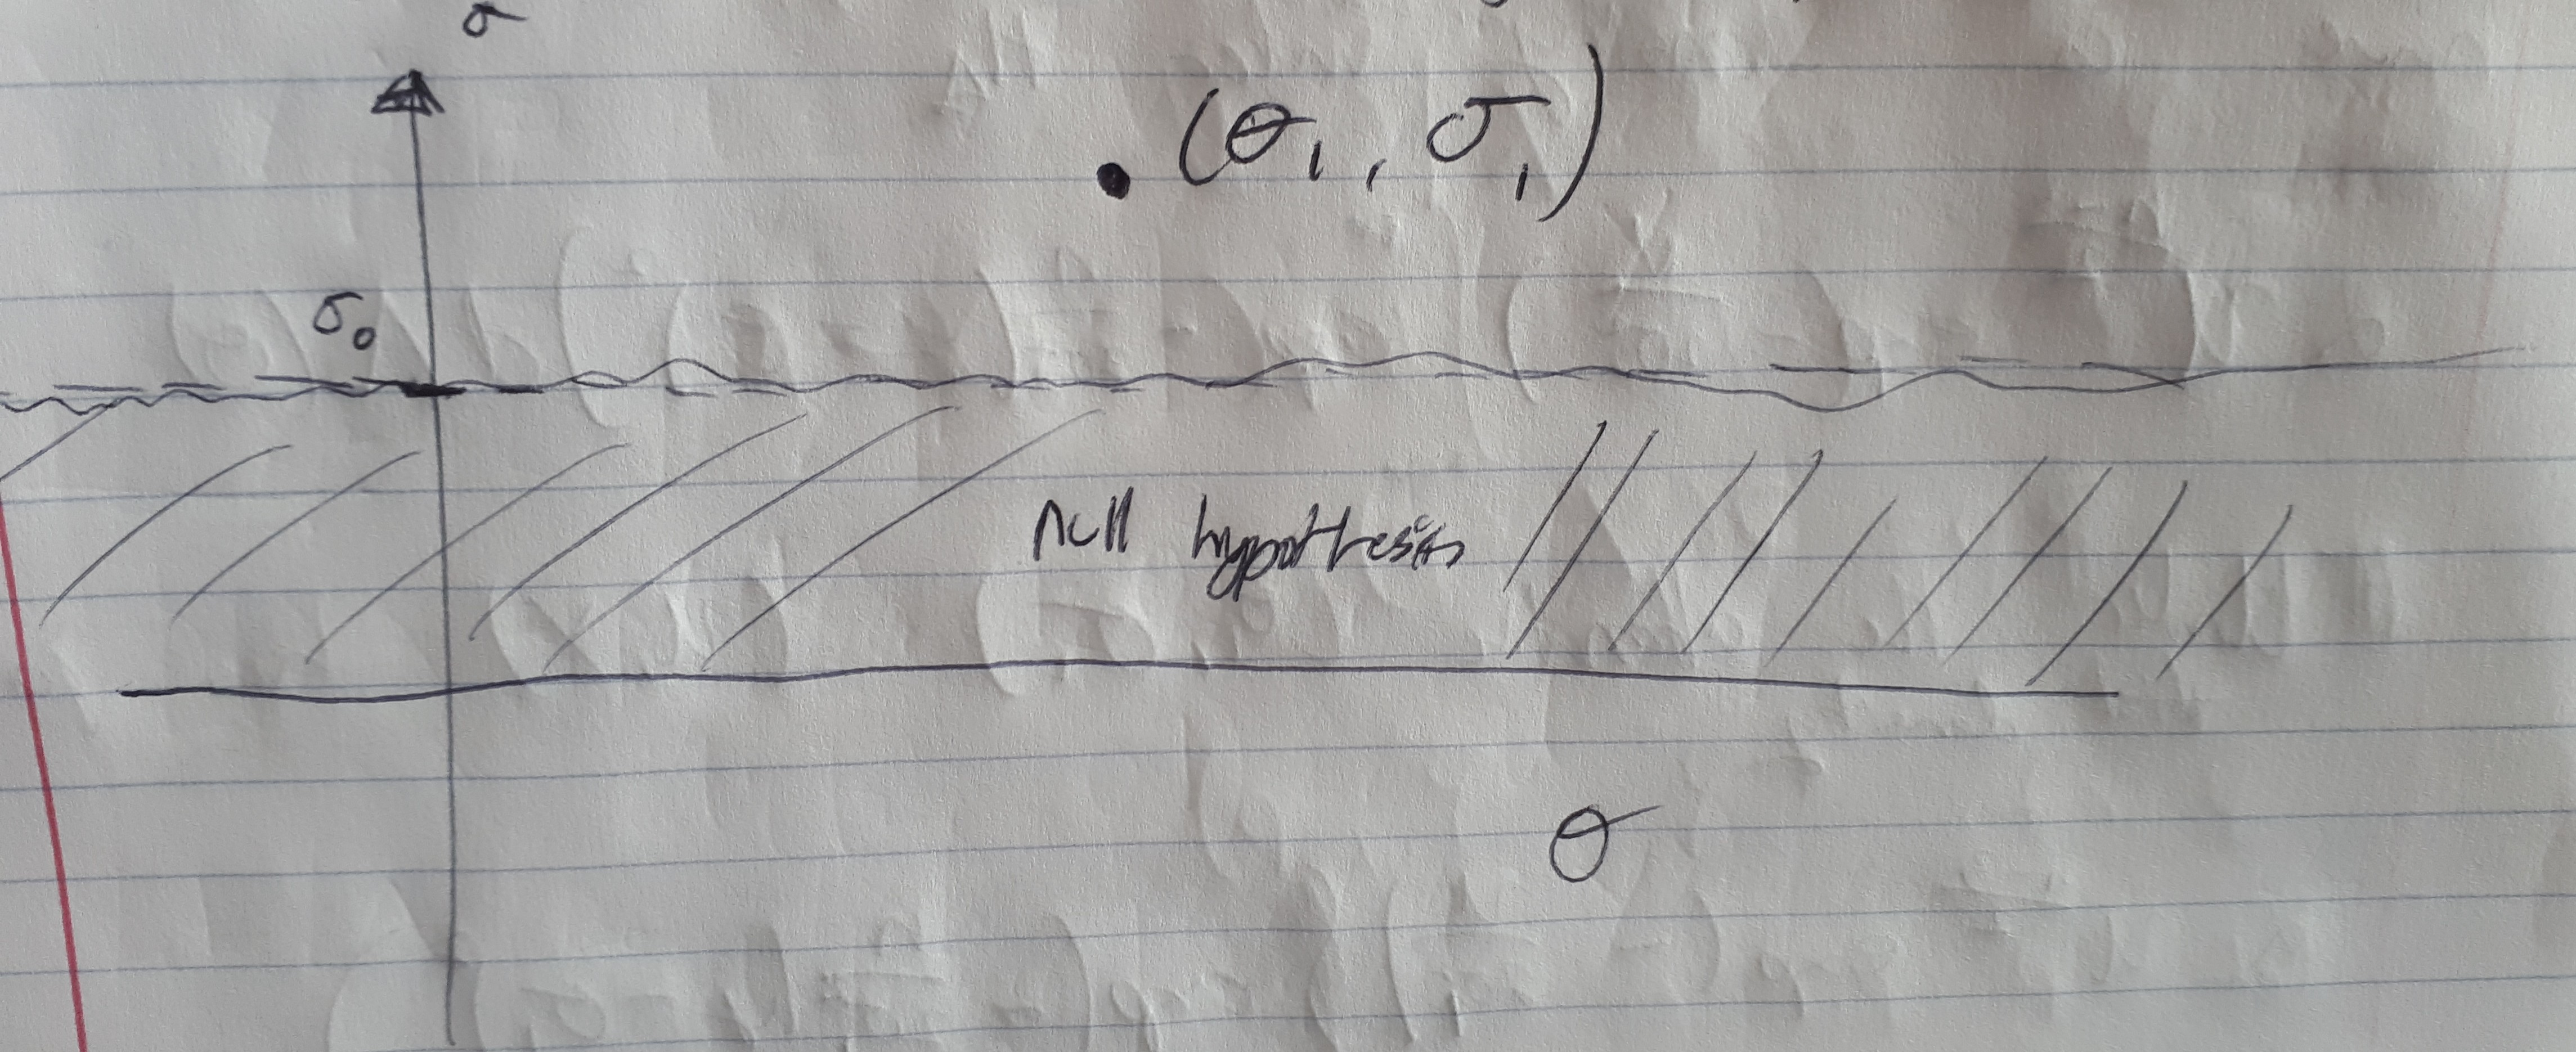
\includegraphics[width = \textwidth]{11_08_P1.jpg}
\end{center}
We have the idea that testing is hard when $\sigma = \sigma_0$ since the $\sigma$ is as close as possible to $\sigma_1$. Thus we guess that our probability distribution $\Lambda$ should be supported on 
\[\{(\ta,\sigma_0):\ta \in \R\}.\] 

We can further simplify things by working with sufficient statistics. This is because if we are given a test function $\phi$ and a sufficient statistic $T$, then we can define a test function $\eta$ given by 
\[\eta(t) = \E[\phi(X)|T=t]. \]
The test function $\eta$ has power and level equal to that of $\phi$ and $\eta$ is a function of only the sufficient statistic $T$. Furthermore $\eta$ is well-defined by sufficiency. 

In our example, a sufficient statistic is
\[(Y,U) = \left(\bar{X}, \sum_{i=1}^n (X_i-\bar{X})^2\right). \]
By Basu's theorem we know that $Y$ and $U$ are independent under any choice of $(\ta,\sigma)$. We also know that $Y \sim \Na(\ta, \sigma^2/n)$ and $U/\sigma^2 \sim \chi^2_{n-1}$. For a fixed simple null $(\ta,\sigma_0)$ we know that the joint distribution of $(U,Y)$ is given by 
\[f(u,y;\ta,\sigma_0)\propto u^\frac{{n-3}}{2} \exb{-\frac{u}{2\sigma_0^2}}\exb{-\frac{n}{2\sigma_0^2}(y-\ta)^2}. \]
Thus if we have a distribution $\Lambda$ on $\{(\ta,\sigma_0): \ta \in \R\}$, then the joint distribution of $(Y,U)$ under $H_\Lambda$ is
\[f(u,y;\ta,\Lambda) \propto u^\frac{n-3}{2}\exb{-\frac{u}{2\sigma_0^2}}\int_{-\infty}^\infty \exb{-\frac{n}{2\sigma_0^2}(y-\ta)^2}d\Lambda(\ta).\]
Under the simple alternative $(\ta_1,\sigma_1)$, $(U,Y)$ has joint density
\[f(u,y; \ta_1,\sigma_1) \propto u^\frac{{n-3}}{2} \exb{-\frac{u}{2\sigma_1^2}}\exb{-\frac{n}{2\sigma_1^2}(y-\ta_1)^2}. \]
We wish to choose a distribution $\Lambda$ so that the above distributions are as close as possible. Under the alternative $(\ta,\sigma)=(\ta_1,\sigma_1)$, we have $Y \sim \Na(\ta,\sigma_1^2/n)$. Under $H_\Lambda$, $Y$ has distribution $Z+\Ta$ where $Z$ and $\Ta$ are independent, $\Ta \sim\Lambda$ and $Z \sim \Na(0,\sigma^2_0/n)$. This last claim can be seen by observing that the distribution of $Y$ under $H_\Lambda$ is given by a convolution. If we let $\Lambda = \Na(\ta_1, \sigma_1^2/n - \sigma_0^2/n)$, then $Y \sim \Na(\ta_1, \sigma_1^2/n)$ under $H_\Lambda$. The likelihood ratio thus simplifies to 
\[\frac{\exb{-\frac{u}{2\sigma_1^2}}}{\exb{-\frac{u}{2\sigma_0^2}}} = \exb{u\left(\frac{1}{2\sigma_0^2}-\frac{1}{2\sigma_1^2}\right)}, \]
which is an increasing function of $u$. Thus the MP test is one which rejects when $U$ is large. Under $H_\Lambda$, $U/\sigma_0^2 \sim \chi^2_{n-1}$. Thus the MP level $\al$ test is given by 
\[\phi(x) = \begin{cases}
    1 & \text{if } \frac{1}{\sigma_0^2}\sum_{i=1}^n (x_i-\bar{x})^2 > k,\\
    0 & \text{else}.
\end{cases} \] 
where $k$ is the $1-\al$ quartile of $\chi_{n-1}^2$. We know have to ask if $\phi$ is MP for $H_0$ against $(\ta,\sigma)=(\ta_1,\sigma_1)$. To do this we have to show that $\phi$ has level $\al$ at $(\ta,\sigma)$ for all $\sigma \le \sigma_0$. This is true since if $X_i$ has variance $\sigma^2 < \sigma_0^2$, then 
\[\frac{1}{\sigma_0^2}\sum_{i=1}^n (x_i-\bar{x})^2 \le \frac{1}{\sigma^2}\sum_{i=1}^n (x_i-\bar{x})^2 \sim \chi^2_{n-1}.\]
Thus the probability of rejection decreases as $\sigma$ decreases. Thus $\phi$ is MP for $H_0$ against the simple alternative $(\ta,\sigma)=(\ta_1,\sigma_1)$. Since $\phi$ does not depend on $(\ta_1,\sigma_1)$ we can conclude that $\ta$ is in fact UMP for $H_0 : \sigma \le \sigma_0$ against $H_1 : \sigma > \sigma_0$. 
\begin{remark}
    One can ask: Why doesn't taking $(\ta,\sigma) = (\ta_1,\sigma_0)$ work? One could argue intuitively that this is the distribution ``closest'' to $(\ta_1,\sigma_1)$. This fails because the MP test of $(\ta,\sigma) = (\ta_1,\sigma_0)$ against $(\ta,\sigma)=(\ta_1,\sigma_1)$ is given by 
    \[\phi_{\ta_1}(x) = \begin{cases}
        1 & \text{if } \sum_{i=1}^n (x_i-\ta)^2 > k,\\
        0 & \text{else}.
    \end{cases} \]
    This test is problematic since it depends on $\ta_1$ but also it is not level $\al$ for the null $H_0 : \sigma \le \sigma_0$. If we let $\ta_1 \to \infty$, the level approaches 1.
\end{remark}
\subsection{Non-parametric quantile test}
Suppose $X_1,\ldots, X_n \iid \Pa \in \Po$ where $\Po$ is the set of all distributions on $\R$. For fixed $\mu \in \R$ and $p_0 \in [0,1]$ we wish to test
\[H_0 : \Pa(X \le \mu) \ge p_0 ~~\text{against}~~H_1 : \Pa(X \le \mu) < p_0. \]
Inuitively, a test which counts the number of $i$'s such that $X_i \le \mu$ might be UMP. To check this consider the following reparametrization: 
\[\Pa \longleftrightarrow (\Pa^-, \Pa^+, p), \]
where 
\begin{align*}
    \Pa^+ &= \text{the conditional distribution of } X \mid X \le \mu,\\
    \Pa^- &= \text{the conditional distribution of } X \mid X > \mu,\\
    p     &= \Pa(X \le \mu).
\end{align*}
There is a correspondence between the triples $(\Pa^+,\Pa^-,p)$ and the distributions $\Pa$. Let $p_-$ and $p_+$ be the densities for $\Pa^-$ and $\Pa^+$, the density of $\Pa$ is thus 
\[p(x) = p\cdot p_-(x) \one_{x \le \mu} + (1-p)\cdot p_+(x)\one_{x > \mu}. \]
If we sort $X_1,\ldots, X_n$ such that 
\[X_{i_1},\ldots, X_{i_m} \le \mu \text{ and } X_{j_1},\ldots,X_{j_{n-m}} \ge \mu, \]
then under a simple alternative $(\Pa^-, \Pa^+,p_1)$ where $p_1 < p_0$, the joint density of $(X_1,\ldots, X_n)$ is 
\[p(x) = p_1^m \prod_{k=1}^m p_-(x_{i_k}) (1-p_1)^{n-m}\prod_{k=1}^{n-m}p_+(x_{j+k}). \]
If we wish to pick distribution which gives us a null which is close to the above distribution we should take $(\Pa_-,\Pa_+,p_0)$. This formalizes the idea that there is ``no information'' in the tails of $\Pa$ and that ``all information'' is contained in $\Pa(X \le \mu)$ which is the quantity we are interested in. When testing the simple null $(\Pa_-,\Pa_+,p_0)$ against the simple alternative $(\Pa_-,\Pa_+,p_1)$, the likelihood ratio is 
\[ \frac{p_1^m(1-p_1)^{n-m}}{p_0^m(1-p_0)^{n-m}},\]
since $p_1 < p_0$ we reject when the quantity 
\[m = \abs{\{i : X_i \le \mu \}}, \]
is small. Under our simple null, $m$ has a binomial $(n,p_0)$ distribution thus the MP test is 
\[\phi = \begin{cases}
    1& \text{if } m < k,\\
    \gamma&\text{if } m=k,\\
    0 & \text{if} m > k.
\end{cases} \]
where $k$ and $\gamma$ are determined by $\E_{p_0}\phi = \al$. 

Note that this test is level $\al$ for the original composite $H_0$. This is because the power function $\beta(\ta)$ depends on $(\Pa^-, \Pa^+,p)$ only through $p$ and the power function is a decreasing funcion of $p$. Thus we can conclude that $\phi$ is MP for the oringal $H_0$. Furthermore $\phi$ does not depend on $(\Pa^-,\Pa^+,p_1)$ and thus $\phi$ is UMP for 
\[H_0 : \Pa(X \le \mu) \ge p_0 ~~\text{against}~~H_1 : \Pa(X \le \mu)>p_0. \]

\end{document}